\lecture{1}{}
\section{Class Group}%
\label{sec:Class Group}
Current group: Group 4: Medicine (4 stus, Ibuprofen)

Group Logo:
\begin{figure}[htpb]
    \centering
    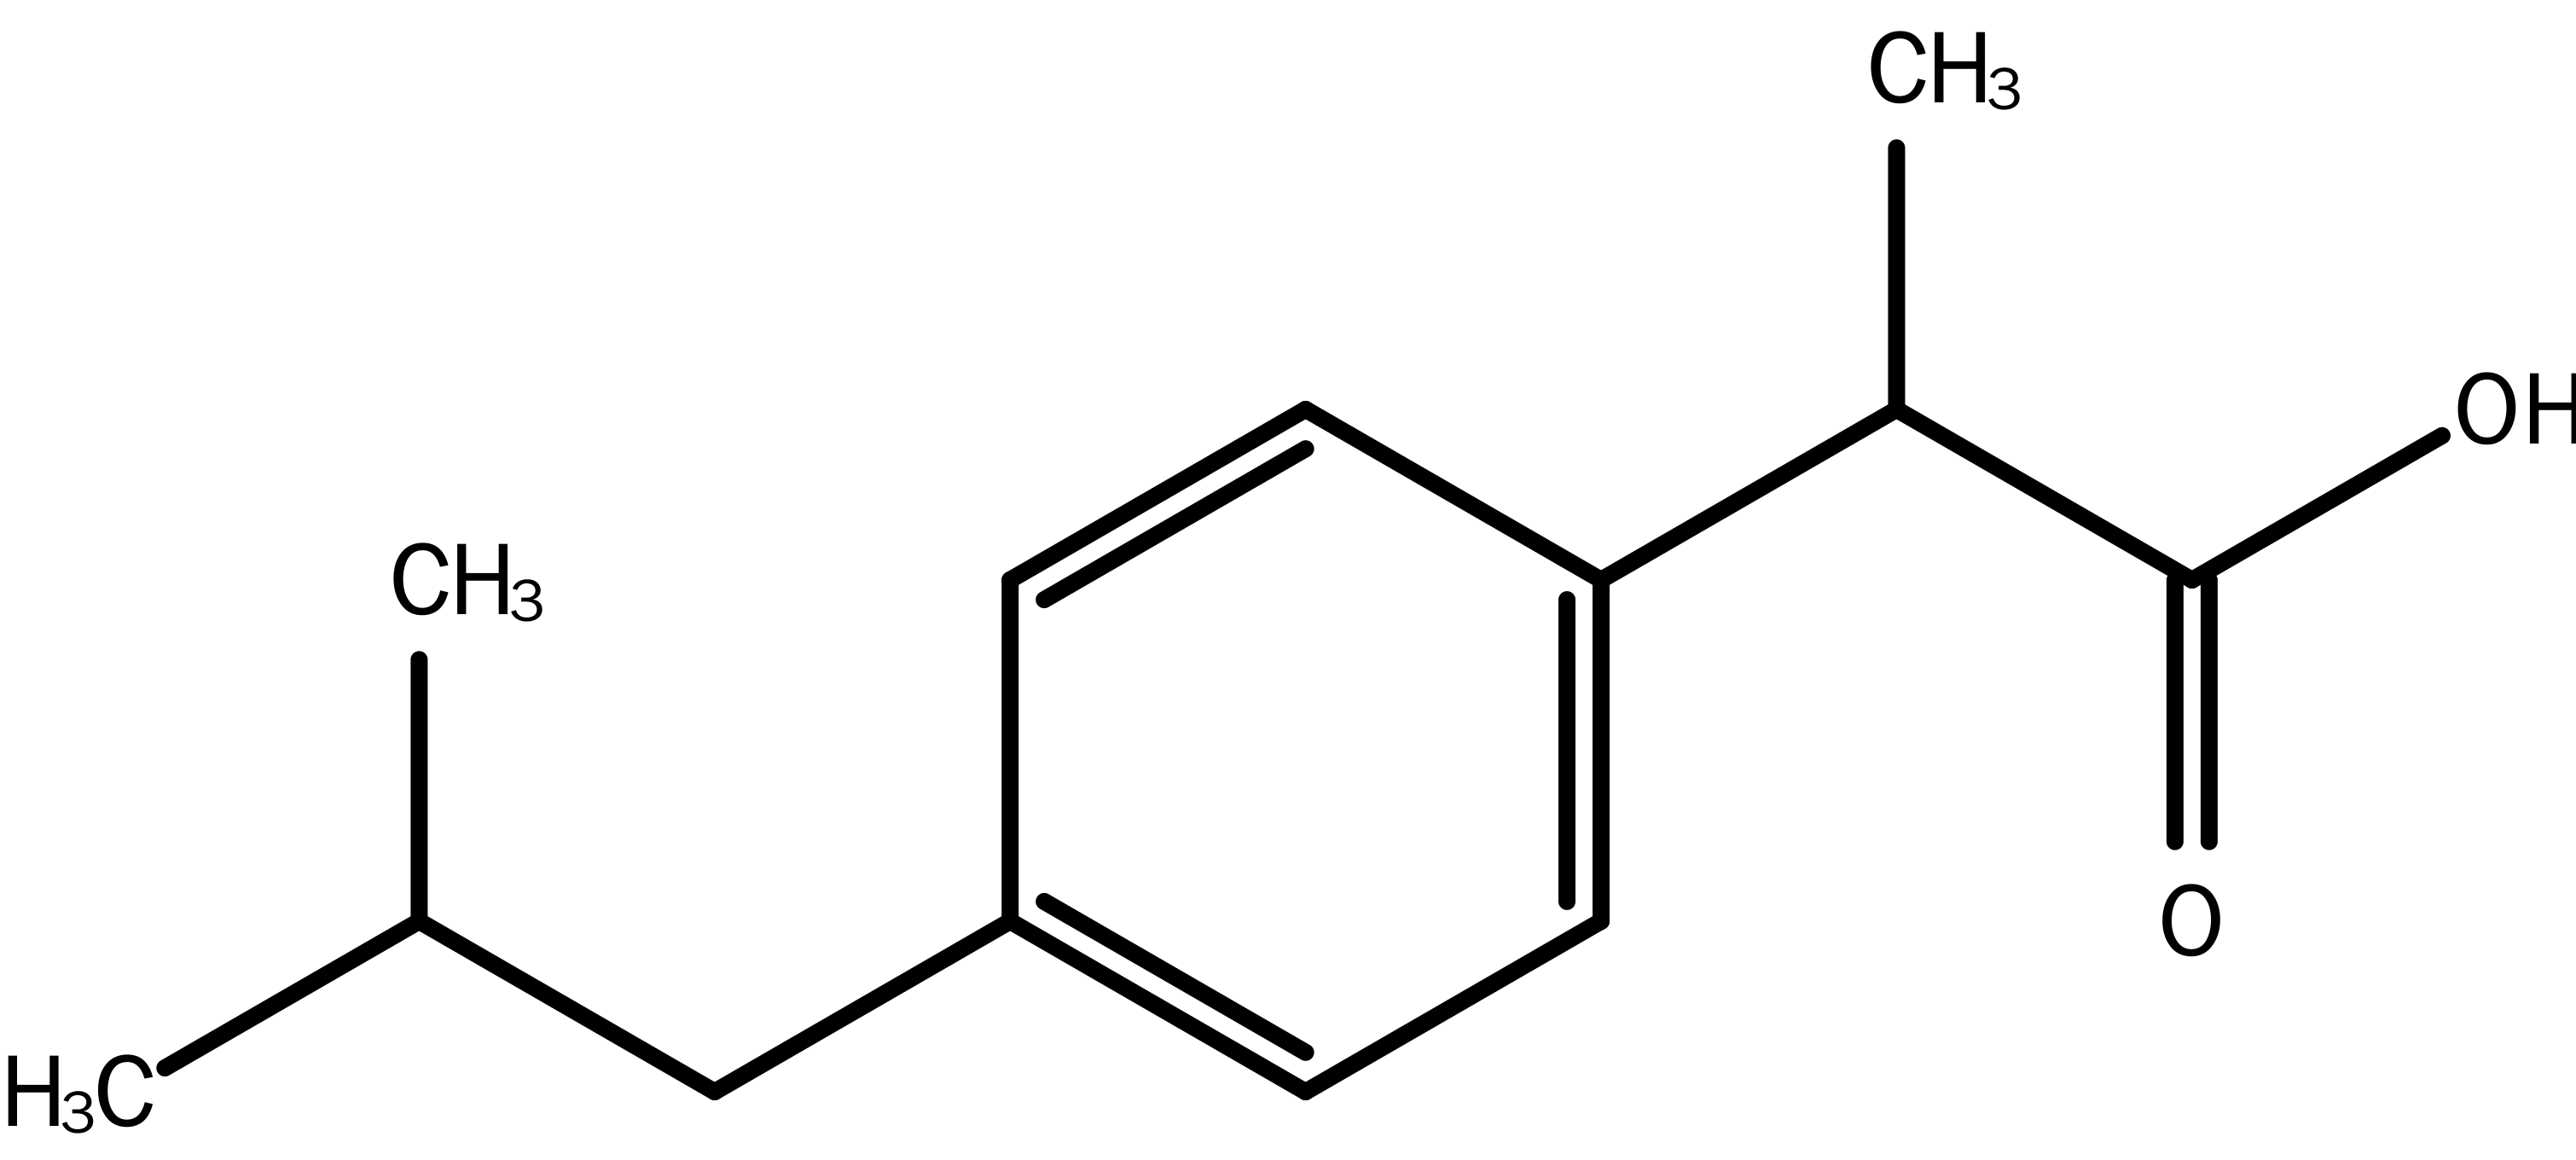
\includegraphics[width=0.5\textwidth]{fig/Ibuprofen}
    \caption{Ibuprofen}
    \label{fig:Ibuprofen}
\end{figure}

Groups:
\[
    \begin{cases}
        \text{Water Supplement: Water Group Six}\\
        \text{Smart Construct: None}\\
        \text{Environment: E5G}\\
        \text{Math: The endless road}\\
        \text{Build environment engineering: The Beechburg}\\
        \text{Engineering: None}\\
        \text{Medicine: Ibuprofen}\\
        \text{Civil engineering: ER}
    \end{cases}
.\] 

The outstanding problem in translation: special word

Activity: Type a message include group name, group members and group number

\section{Search for Papers}%
\label{sec:Search for Papers}
How to Search Papers:

1. Key words in paper you want to check: Decide key word in major (in medicine)

2. Enter Web of Science or other paper check website (Web of Science is a search-only database)

3. ? 

\begin{notation}
    How a green hand gradually become a veteran?

    1. Hard working

    2. A good teacher and famous people to be teached for

    3. Participate in great communities
    
    4. Get a mysterious success key
    \begin{eg}
        Sun WuKong, Wei XiaoBao, GuoJing
    \end{eg}
\end{notation}
\begin{notation}
    How to be stronger in my major?

    1. Hard working

    2. A good teacher and a leader

    3. High quality papers

    4. Good commities to join
\end{notation}
\begin{notation}
    A project is based on sponsors, generally based on money
\end{notation}
\begin{notation}
    If you want to make yourself stronger:

    1. Write paper

    2. Get sponsor to do exps

    3. Make price/patent application

    4. Get rich
\end{notation}
In this term stus can apply for a new project, then apply for sponses, do experience to make something new, write paper, apply for patent, then in term V you can become a person decorate with amazing characteristics. After term VI there will be a summer camp, with these parts you will quickly get into famous.

    Destination is to see what famous people have done and follow them: their sponsors, the communities they join and papers they have published (to get the journals and conferences they choose)

    JCR stands for the level this journal is, divided into 4 levels

    When we are not familiar with a new field, we can check into a famous person in this field, while we can also settle our growing path and get important journals/commities quickly

\begin{notation}
    Famous researchers in domestic Medicine: 

    Famous journals in Medicine: Journal of Controlled Release
\end{notation}

After Class Homework: see 3 top journals, check catalog in these journals, find 10 recently research project in current major
